\documentclass[a4paper,11pt]{article}
\usepackage[T1]{fontenc}
\usepackage[utf8]{inputenc}
\usepackage{lmodern}
% \usepackage{hyperref} % fucking warnings
\usepackage{graphicx}
\usepackage{graphics}
\usepackage{rotating}
\usepackage{listings}
\usepackage{color}
\usepackage{listings}
\usepackage{amsthm}
\usepackage{amsmath}
\usepackage{amssymb}
\usepackage{algorithmic}
\usepackage{datatool}
\usepackage{caption}
\usepackage{subcaption}

% \newcommand{\encode}[1] {{ {}_{\llcorner}{#1}_{\lrcorner}}}

\title{Numerical Linear Algebra (CSE-6643) - Final take home exam}
\author{Arash Rouhani (rarash@gatech.edu) - gtid: 902951864}


\begin{document}

\maketitle

\section{Part I}

% This task consists of (1) discretizing a differential equation into
% linear equation, (2) solving the linear equation using own
% written gauss elimination and (3) plotting,  timing and commenting on
% results.

\subsection{Method}

I used power iteration to find the largest eigenvalue and inverse iteration to
find the smallest. There is really no reason for not using the inverse
iteration for both. One could have used one for the other but I wanted to try
both.  I also used the rayleigh quotient iteration to see how much better it
performs. But first, lets recap how I discretize the problem.

\subsubsection{Discretization (exactly as previous project)}

For $n$ interior points we have $m=n+1$ interior slices. We define $h$
to $1/m$ which is the distance between the points. With this a natural
discretization appears

\[
  u''[i] = \frac{1}{2} - \frac{i}{m} = \frac{u[i+1]-2u[i]+u[i-1]}{h^2}
\]

Where $u$ is unknown, of course, we want to solve for it since it's a
differential equation. More precisely, $u[0]=u[m]=0$ are corresponding
to the given initial values and $u[i]$ exists for $i = 1..n$.

Now we want to form the typical equation $Ax=b$ such that solving for
$x$ gives all $u[i]$. The equation above gives us this scheme: Let $A$
be a tridiagonal matrix with only $-2$ in the diagonal and $1$ in its
sub- and super diagonal. Set $b_i$ to $(1/2-i*h)h^2$. $x_i$ is simply
$u[i]$ in this scheme.


\subsubsection{Power Iteration (PI)}

I implemented the version in the course book.  $e_1$ was set to the
initial guess of eigenwector since I didn't find any analysis that
motivated that taking any particular normal vector would help the
convergence of the algorithm.

To actually retrieve the largest eigenvalue from the vector that power
iteration returns, you just take the rayleigh quotient of that vector.
Note that the vector should hopefully be coverging to the eigenvector
corresponding to the largest eigenvalue.

\subsubsection{Inverse Iteration (II)}

Again I decided to use $e_1$ as my eigenvector guess $v^{(0)}$.  Unlike
when using Power Iteration, some understanding about $A$ is required, I
must provide an eigenvalue close to the one I want. In order to find a
value that always is close to the smallest eigenvalue I decided to
experiment with $A$ for various $n$. My conclusion was that the smallest
eigenvalue is approaching $0.0$ as $n$ increases. Therfor $\mu=0.0$ is
reasonable.

\subsubsection{Rayleigh Quotient Iteration (RQI)}

While the book again provided most of the guidance, to arbitrarily pick
a vector like $e_1$ as initial guess is not possible since this
iteration will actually converge to the eigenvector closest to your
guess. Also, even though I know that the eigenvalues always seem to be
within the range $(0.0, 4.0)$, I must in fact know a
eigen\emph{vector} estimate this time.

By experimenting like I did when deciding $\mu$ for inverse iteration, I
came up with this scheme for constructing an eigenvector like the one
corresponding to the smallest eigenvalue. That eigenvector is in a
pattern like this $normalize([4, 5, 6, 7, 7, 6, 5, 4])$ for $n=8$.  This
pattern is easy to model programtically. The corresponding eigenvector
for largest eigenvalue is the same only with alternating signs.

\subsubsection{Termination conditions}

As for PI, I found it hard to construct a sensible termination condition
without polluting the results, so I decided to use a fixed number of
iterations. The II continues until the improvement becomes smaller than
$10^{-14}$. The Rayleigh Quotient termination condition was tricky.
Intuitively one should keep iterating while $M=A-\lambda^{(k)}I$ is "very
nonsingular", which corresponds to having a determinant that is bigger
than some constant. But that turned out to not work because of rounding
issues. The determinant won't go below a certain limit and that limit
increases with $n$, hence the constant that decides if the determinant
is small enough has to increase with $n$. One such value that worked out
was $\kappa(A)10^{-10}$. I noted that no matter what limit I tried I
never got beyond two iterations though! See table \ref{tab:conda} for
the condition numbers

\subsubsection{Sparsity}

I will not demonstrate any evidence here, but I used matlabs sparse
matrices everywhere to \emph{massively} improve the performence and
allowing larger $n$ to be tried out. So it indeed was not any fancy
hardware that allowed for a large $n$, rather, it was a good algorithm.

\subsubsection{Condition number}

I used the condition number estimate \texttt{condest} in matlab that can
use the fact that the matrix is sparse to estimate the condition number
quickly.

\newcommand{\fornTwo}[1] {
  #1{100}
  #1{200}
}

\newcommand{\fornSix}[1] {
  \fornTwo{#1}
  #1{400}
  #1{800}
  #1{1600}
  #1{3200}
}

\newcommand{\fornEight}[1] {
  \fornSix{#1}
  #1{6400}
  #1{12800}
}

\newcommand{\fornTen}[1] {
  \fornEight{#1}
  #1{25600}
  #1{51200}
}

\newcommand{\pimacro}[1] {
  \ensuremath{n=#1} & \input{data/1-pi_conv_ratio-#1.dat}
                    & \input{data/1-diff_largest-#1.dat}
                    & \input{data/1-it_l-#1.dat}
                    \\ \cline{2-4}
}
\begin{table}[h]
  \centering
  \begin{tabular}{r|c|c|c|}
    \multicolumn{1}{r}{}
     & \multicolumn{1}{c}{$1-{\lambda_2}_{ML}/{\lambda_1}_{ML}$}
     & \multicolumn{1}{c}{${\lambda_1}_{ML}-{\lambda_1}_{PI}$}
     & \multicolumn{1}{c}{$iterations_{PI}$}\\
    \cline{2-4}
    \fornEight{\pimacro}
  \end{tabular}
  \caption{Power iteration to get the largest eigenvalue}
  \label{tab:powerit}
\end{table}

\newcommand{\iimacro}[1] {
  \ensuremath{n=#1} & \input{data/1-diff_smallest-#1.dat}
                    & \input{data/1-it_s-#1.dat}
                    \\ \cline{2-3}
}
\begin{table}[h]
  \centering
  \begin{tabular}{r|c|c|}
    \multicolumn{1}{r}{}
     & \multicolumn{1}{c}{${\lambda_n}_{ML}-{\lambda_n}_{II}$}
     & \multicolumn{1}{c}{$iterations_{II}$}\\
    \cline{2-3}
    \fornTen{\iimacro}
  \end{tabular}
  \caption{Inverse iteration to get the smallest eigenvalue}
  \label{tab:inverit}
\end{table}

\newcommand{\rqimacro}[1] {
  \ensuremath{n=#1} & \input{data/1-diff_rq_largest-#1.dat}
                    & \input{data/1-it_rq_l-#1.dat}
                    & \input{data/1-diff_rq_smallest-#1.dat}
                    & \input{data/1-it_rq_s-#1.dat}
                    \\ \cline{2-5}
}
\begin{table}[h]
  \centering
  \begin{tabular}{r|c|c|c|c|}
    \multicolumn{1}{r}{}
     & \multicolumn{1}{c}{${\lambda_1}_{ML}-{\lambda_1}_{RQI}$}
     & \multicolumn{1}{c}{$iterations_{RQI}$}
     & \multicolumn{1}{c}{${\lambda_n}_{ML}-{\lambda_n}_{RQI}$}
     & \multicolumn{1}{c}{$iterations_{RQI}$}\\
    \cline{2-5}
    \fornTen{\rqimacro}
  \end{tabular}
  \caption{Rayleigh quotient iteration to get both the extreme eigenvalues}
  \label{tab:rqit}
\end{table}

\newcommand{\condamacro}[1] {
  \ensuremath{n=#1} & \input{data/1-cond_A-#1.dat}
                    & \input{data/1-my_cond_A-#1.dat}
                    \\ \cline{2-3}
}
\begin{table}[h]
  \centering
  \begin{tabular}{r|c|c|}
    \multicolumn{1}{r}{}
    & \multicolumn{1}{c}{$\kappa(A)_{ML}$}
     & \multicolumn{1}{c}{${\lambda_1}_{RQI}/{\lambda_n}_{RQI} $} \\
    \cline{2-3}
    \fornTen{\condamacro}
  \end{tabular}
  \caption{Condition number of $A$}
  \label{tab:conda}
\end{table}

\subsection{Results and explenations}

% There are some observations that are interesting whilst others aren't. 

In the tables, $\lambda_1$ and $\lambda_n$ is the largest and the
smallest eigenvalues respectively. They of course vary with $n$. We also
consider it to be known fact that they approach $4.0$ and $0.0$
as $n$ grows. I also compare my values to the eigenvalues
returned by Matlab's \texttt{eig} function. For instance
${\lambda_1}_{ML}$ is the biggest of the eigenvalues that matlab finds.

\subsubsection{Accuracy}

The power iteration isn't that impressive and it's clear that the values
are far away from the correct (matlab's) answer. Furthermore, for most
$n$ the values start converging extremely slow at about $0.003$. If you
drastically increase the number of iterations the accuracy will improve.

But for inverse iteration and rayleigh quotient iteration things are not
as obvious. Is matlab right or is any of my implementations closer to
the right answer? On one hand matlab is a high quality software but at
the same time it was instructed to find all eigenvalues but I only aimed
for a more specialized task which is obviously easier. No matter what
both those two iterations are extremely close to matlabs answer and each
other. It's therfor obvious that they work as they should.

\subsubsection{Comparing Inverse iteration with Power iteration}

Theoretically, increasing $n$ works in the favor of inverse
iteration but against power iteration. In the Inverse iteration
case, our lowest eigenvalue estimate $\mu=1.0$ is getting closer and
closer to the actual lowest eigenvalue when $n$ increases. However, for
power iteration, an increasing $n$ means that the convergence factor
$\lambda_2/\lambda_1$ decreases which makes power iteration requiring
more and more iterations to achieve the same accuracy. Both these
theoretical observations are confirmed in table \ref{tab:powerit}
and \ref{tab:inverit}.

\subsubsection{Only two iterations!?}

The speed of the rayleigh quotient is astonishing. The theoretical
explanation is that it's convergence is cubic. See table
\ref{tab:rqit}.

\subsubsection{Ill conditioned ness}

Since $\kappa(A) = \lambda_{max}/\lambda_{min}$ in general for a
hermitian matrix I accompany matlabs estimate with the divsion of the
calculated eigenvalues from my rayleigh quotient iteration. See table
\ref{tab:conda}. Note that the values are different as matlab calculates
the first norm condition number.

% \newcommand{\genfig}[3] {{
%     \begin{figure}
%             \centering
%             \begin{subfigure}[b]{1.0\textwidth}
%                     \includegraphics[width=\textwidth]{fig/#1-#2-100}
%                     \caption{$n = 100$}
%             \end{subfigure}
%             \begin{subfigure}[b]{1.0\textwidth}
%                     \includegraphics[width=\textwidth]{fig/#1-#2-150}
%                     \caption{$n = 150$}
%             \end{subfigure}
%             \caption{Medians of the columns of $\Delta #2$ #3}\label{fig:#1-#2}
%     \end{figure}
%   }}


\section{Part II}

Before anything lets just rewrite the equation to form that is easier to
reason about

\[
  \lambda u(x) - a'(x)u'(x) - a(x)u''(x) = x - \frac{1}{2}
\]

\subsection{Method}

Again

\subsubsection{Discretization}

We note that $b$ and $x$ of our $Ax=b$ discretization are just like for
Part I.  However, $A$ will be different. To construct $A$, we start by
recalling the centered difference scheme (this is one way of doing it,
see discussion of the symmetricity constraint).

\[
  u[i] = u[i]
\]
\[
  u'[i] = \frac{u[i+1]-u[i-1]}{2h}
\]
\[
  u''[i] = \frac{u[i+1]-2u[i]+u[i-1]}{h^2}
\]

The differential equation's LHS is just a combination of these
three kinds of variables which all can be expressed in $u[i]$ and
hence be factored out to be the $x$ part of $Ax=b$. To actually
construct $A$ is now doable, it's just the sum of three matrices
corresponding for the three terms $u[i]$, $u'[i]$ and $u''[i]$. $A$ will
again be tridiagonal. The diagonal will be affected by the $u[i]$ term
and the $u''[i]$ term while the two outer diagonals will be affected by
$u'[i]$ term and again the $u''[i]$ term. The matrix term corresponding
to the $u[i]$ part is $\lambda I$ where $I$ is the $n$ by $n$ identity
matrix.

\subsubsection{The constraints and resolving of violations}

Both steepest descent and the conjugate gradients method require
$A$ to be hermitian and positive semidefinite. Lets investigate!

\paragraph{The Positive Definite Constraint}

A requirement for both Steepest descent and conjugate gradient is that
the matrix $A$ in $Ax=b$ is Positive definite. I checked by construction
that all matrices are positive definite, so luckily it doesn't impose
any problem.

\paragraph{The symmetry constraint}

For the $a(x) = 2$ it's obvious that $A$ is symmetric as the whole
$u'(x)$ term will be canceled out by $a'(x) = 0$. Studying the
discretized symmetric difference equations reveals that only the $u'[x]$
equation will cause an imbalance since the term in front of $u''(x)$
(that is $a(x)$) will only be the constant $2$. But at a first glance
one might expect to not be as lucky when $a(x) = x$ since now the
$u'(x)$ will be part of $A$.  Yet now also the $u''(x)$ term is affected
since $a(x)$ is no longer a constant. By doing the math one can prove
that $A_{(i+1)i} = A_{i(i+1}$.

Hence, the symmetric difference scheme you use will have an enormous
impact. If for instance you let the $u''(x)$ term affect
$A_{i(i+2)}=A_{(i+2)i}$ instead of $A_{i(i+1)}=A_{(i+1)i}$ you deal with
the issues of $A$ not being symmetric and CG nor SD could be applied
directly.

\paragraph{If we wouldn't be as lucky}

The fact that the matrix always turned out to be symmetric is nothing
but a miracle. Would got not have blessed us in our calculations, one
would have been able to try to solve the system $A^{*}Ax=A^{*}b$ since
$A^*A$ is always positive definite and symmetric.  It even gets carried
out in linear time for tridiagonal $A$! But one will suffer a squaring
of the condition number making the new equation system much more ill
conditioned.

\subsubsection{Steepest Descent (SD) and Conjugate Gradients (CG)}

The only interesting parts of these algorithms is the termination
conditions. It can be proven that the SD method will converge in
$O(\kappa(A))$ steps and CG only need the square root of that.
I'll let SD run for exactly $\kappa(A)$ iterations and CG run for
$\sqrt{\kappa(A)}$ iterations.

\subsection{Results and Comments}

It's very clear from the graphs that neither algorithm did converge to
what it's supposed to. Not only are the graphs for various $n$ quite
different, but across the algorithms the they've almost clustered.

We notice a couple of details here. First, a large $\lambda$ decreases the
condition number of $A$. Compare table \ref{tab:ct-id-1000} and
\ref{tab:ct-id-1}. As an effect in those tables, the execution time is
much better as the conditioning of $A$ is better (for every $n$). Of
course this is because the way we choose the termination condition of
the two algorithm. Yet we did have a very sound reasoning when choosing
those conditions and I bet high quality software has similar termination
conditions (albeit they do preconditioning and use other cool tricks).

Furthermore, in the cases where the condition number is small, which is
when either $\lambda$ is large or simply when $n$ is small, the
performence of the SD isn't worse than that of CG. However, as the
condition number grows, the execution time for SD becomes unbearable while
the CG time is still faster than human perception.

Just like in Part 1 We observe that the condition number increases at
the same rate as the number of elements in the Array. In part 1 it
were bad because of the arithmetical errors that made the termination
conditions for rayleigh quotient difficult. Here, it means that
\emph{the execution time of conjugate gradients increase linearly with
$n$ for the same sort of matrices}


\newcommand{\ctentries}[3] {
  \ensuremath{n=#3} & \input{data/2-#1-#2-cond_estimate-#3.dat}
                    & \input{data/2-#1-#2-time_sd-#3.dat}
                    & \input{data/2-#1-#2-time_cg-#3.dat}
                    \\ \cline{2-4}
}

\newcommand{\cttable}[2] {
  \begin{table}[h]
    \centering
    \begin{tabular}{r|c|c|c|}
      \multicolumn{1}{r}{}
      & \multicolumn{1}{c}{\ensuremath{\kappa(A)}}
       & \multicolumn{1}{c}{Time for SD (seconds)}
       & \multicolumn{1}{c}{Time for CG (seconds)}\\
      \cline{2-4}
      \fornSix{\ctentries{#1}{#2}}
    \end{tabular}
    \caption{Table with \ensuremath{a(x)} being the #1 function and
    \ensuremath{\lambda = #2}}
    \label{tab:ct-#1-#2}
  \end{table}
}

\cttable{const}{100}
\cttable{const}{10}
\cttable{const}{1}
\cttable{const}{-1}
\cttable{id}{1}
\cttable{id}{10}
\cttable{id}{100}
\cttable{id}{1000}

% These method both have a straight forward implementation when pseduo
% code is provided (CG is in the book and SD 


\newcommand{\genfig}[2]{
    \centering
    \begin{figure}
      \includegraphics[width=\textwidth]{fig/2-#1-#2-u.png}
      \caption{Figure with \ensuremath{a(x)} being the #1 function and
    \ensuremath{\lambda = #2}}
      \label{fig:#1-#2}
    \end{figure}
}


\genfig{const}{100}
% \genfig{const}{10}
% \genfig{const}{1}
% \genfig{const}{-1}
% \genfig{id}{1}
% \genfig{id}{10}
% \genfig{id}{100}
% \genfig{id}{1000}






% \begin{figure}
%         \begin{subfigure}[b]{1.0\textwidth}
%           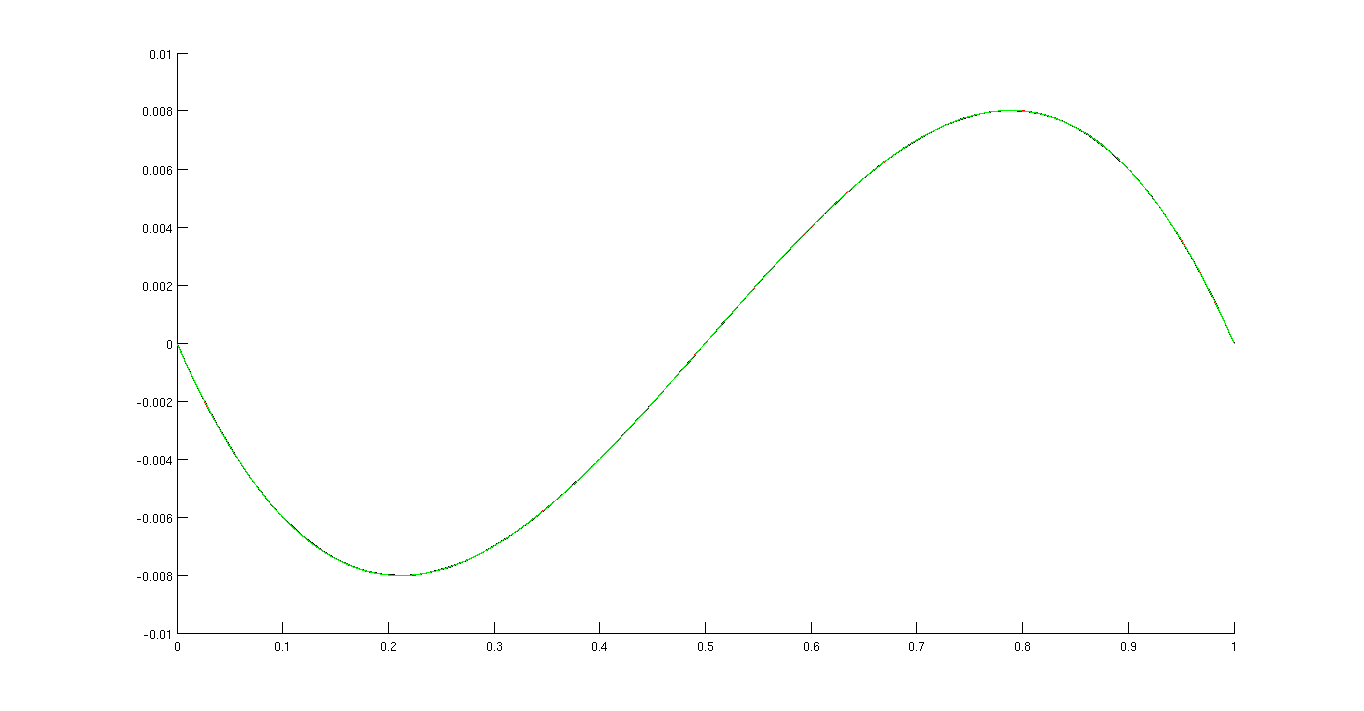
\includegraphics[width=\textwidth]{fig/all.png}
%           \caption{The whole plot}\label{fig:wholeplot}
%         \end{subfigure}

%         \begin{subfigure}[b]{1.0\textwidth}
%           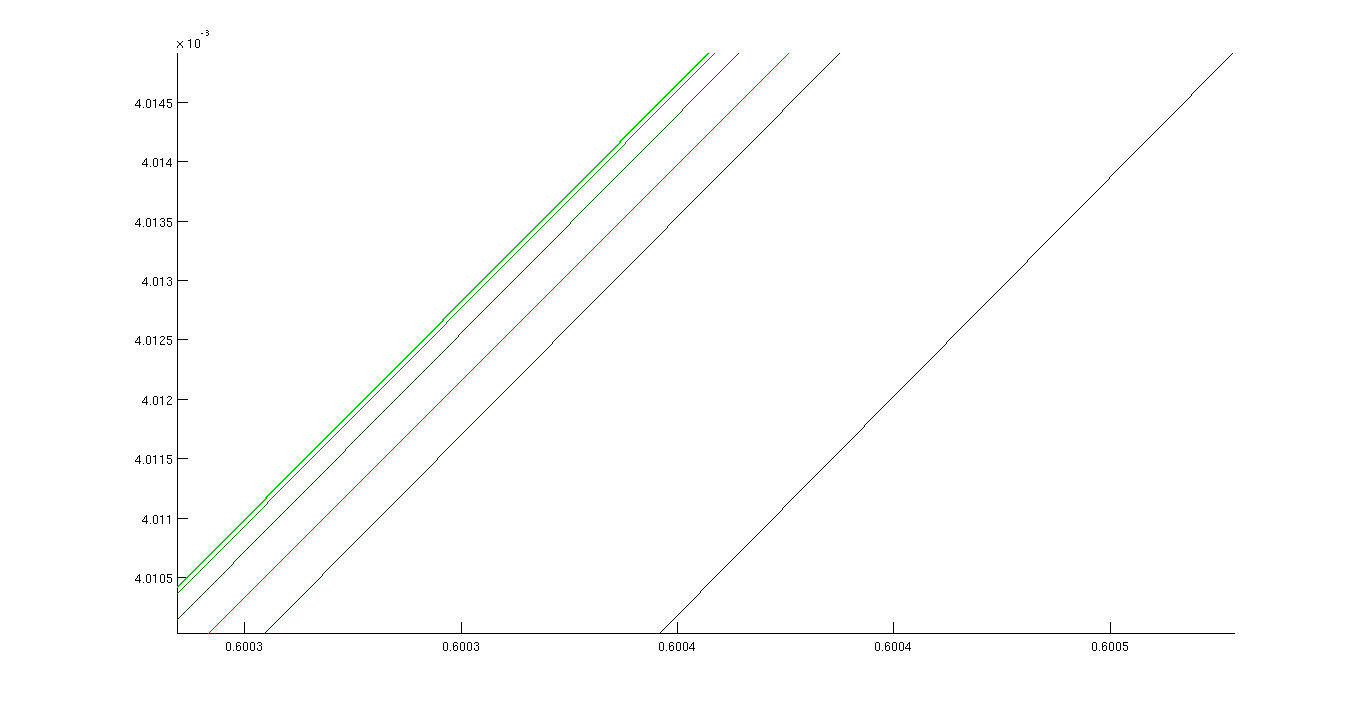
\includegraphics[width=\textwidth]{fig/azoom.png}
%           \caption{One zooming}\label{fig:zooming}
%         \end{subfigure}
%         \caption{Plots of $u(x)$. The red line is the actual function.
%         The others are estimations. The greener the line the higher
%       $n$.}\label{fig:plots}
% \end{figure}


% \section{Table example}

% \begin{table}[h]
%   \begin{tabular}{r|c|c|c|}
%     \multicolumn{1}{r}{}
%      & \multicolumn{1}{c}{$Q_{classic}$ }
%      & \multicolumn{1}{c}{$Q_{stable}$}
%      & \multicolumn{1}{c}{$Q_{householder}$} \\
%     \cline{2-4}
%     $n=100$ & \input{data/norm-q-classi-100.dat}
%             & \input{data/norm-q-stable-100.dat}
%             & \input{data/norm-q-househ-100.dat}
%             \\ \cline{2-4}
%     $n=150$ & \input{data/norm-q-classi-150.dat}
%             & \input{data/norm-q-stable-150.dat}
%             & \input{data/norm-q-househ-150.dat}
%             \\ \cline{2-4}
%   \end{tabular}
%   \caption{Norms for the different unitary $Q$ matrices}
%   \label{tab:norms}
% \end{table}

% \begin{table}[h]
%   \begin{tabular}{r|c|c|c|}
%     \multicolumn{1}{r}{}
%      & \multicolumn{1}{c}{$Q_{classic}$ }
%      & \multicolumn{1}{c}{$Q_{stable}$}
%      & \multicolumn{1}{c}{$Q_{householder}$} \\
%     \cline{2-4}
%     $n=100$ & \input{data/std-q-classi-100.dat}
%             & \input{data/std-q-stable-100.dat}
%             & \input{data/std-q-househ-100.dat}
%             \\ \cline{2-4}
%     $n=150$ & \input{data/std-q-classi-150.dat}
%             & \input{data/std-q-stable-150.dat}
%             & \input{data/std-q-househ-150.dat}
%             \\ \cline{2-4}
%   \end{tabular}
%   \caption{The standard deviation for the values of $A-QR$}
%   \label{tab:stds}
% \end{table}

% \newcommand{\genfig}[3] {{
%     \begin{figure}
%             \centering
%             \begin{subfigure}[b]{1.0\textwidth}
%                     \includegraphics[width=\textwidth]{fig/#1-#2-100}
%                     \caption{$n = 100$}
%             \end{subfigure}
%             \begin{subfigure}[b]{1.0\textwidth}
%                     \includegraphics[width=\textwidth]{fig/#1-#2-150}
%                     \caption{$n = 150$}
%             \end{subfigure}
%             \caption{Medians of the columns of $\Delta #2$ #3}\label{fig:#1-#2}
%     \end{figure}
%   }}

% \genfig{log-median-col}{Q}{logarithmized}
% \genfig{median-row}{Q}{}
% \genfig{log-median-col}{R}{logarithmized}
% \genfig{log-median-row}{R}{logarithmized}


\end{document}
